\chapter{Détection d'objets et apprentissage profond}
\newpage
\pagestyle{fancy}
\fancyhead[L]{\chaptername \ \thechapter}
\fancyhead[R]{Détection d'objets et apprentissage profond}
\renewcommand{\headrulewidth}{1pt}
\fancyfoot[C]{\thepage}
\section{Introduction} 
Au début de l'intelligence artificielle avec la limitation des ressources de calcul, les chercheurs ou les programmeurs devaient choisir et extraire manuellement les caractéristiques, puis appliquer un algorithme tel que la régression ou la classification en fonction des caractéristiques extraites. Cela a limité les performances des modèles et ses résultats en raison des capacités limitées d'un humain à extraire les bonnes caractéristiques, en particulier lorsque les données contiennent une grande quantité de caractéristiques à extraire, ce qui affecte considérablement les performances des modèles.

Avec l'augmentation drastique de la puissance de calcul du matériel moderne, cela a permis d'implémenter un nouvel algorithme qui a résolu le problème précédent d'extraction de caractéristiques et a également créé un nouveau domaine d'intelligence artificielle qui est l'apprentissage en profondeur.

L'apprentissage en profondeur est basé sur des réseaux de neurones avec de nombreuses couches cachées qui, à leur tour, effectuent l'extraction de caractéristiques avec l'objectif du modèle (comme la classification). La première couche du réseau de neurones qui est la couche d'entrée (certains ne l'appellent pas une couche car elle ne contient aucun neurone). Cette couche transmet les données à la couche suivante où résident réellement des neurones, chaque neurone reçoit 1 ou plusieurs entrées de la couche précédente, puis applique un algorithme de calcul tel que : Régression linéaire \(Z = W * X + b\) où w est le poids ou Convolution : \(Z = X * f\) où les valeurs X du noyau sont les poids du neurone. Après avoir calculé Z, la valeur est transmise à une fonction d'activation spécifique telle que : \(ReLu(x) = max(0,x)\) puis la valeur finale est transmise en tant qu'entrée pour la couche suivante jusqu'à ce qu'elle atteigne la couche finale qui produit la prédiction du modèle. Ces étapes sont appelées propagation vers l'avant là où le modèle prédit. 

D'autre part, la rétroporpagation où le modèle apprend, il fait que l'erreur après avoir calculé en comparant les sorties souhaitées aux sorties du modèle prédites, puis en la propageant aux couches précédentes où, pour chaque neurone, les poids sont ajustés en fonction de l'algorithme d'optimisation choisi comme : Gradient Descent.
\begin{figure}[H]
     \centering
     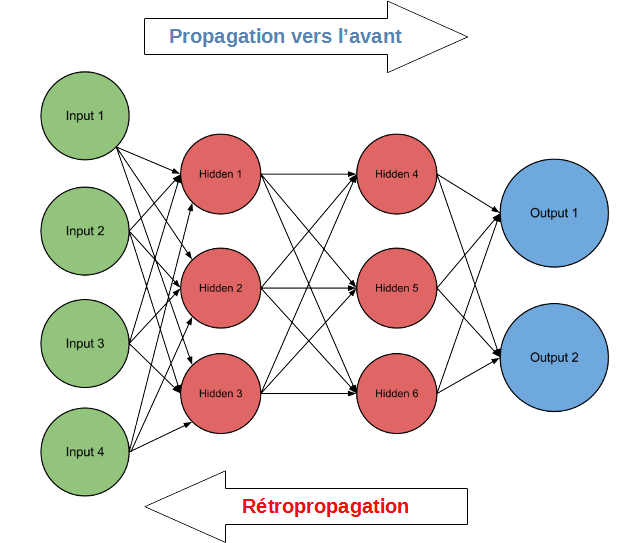
\includegraphics[height=12cm,width=12cm]{Chapitre2/img1.png}
     \caption{Structure d'un réseaux de neurones.}
     \label{img1}
     \end{figure}

\section{Concepts de base} 
% =========== CNN =========== 
     \subsection{Les réseaux de neurones convolutifs (CNN)} 
     De nombreux types de réseaux de neurones sont apparus pour résoudre des problèmes spécifiques, l'un d'eux est le réseau de neurones convolutifs (CNN), un réseau de neurones bien adapté pour traiter des tâches liées à la vision comme la reconnaissance d'objets. Ils ont été introduits pour la première fois en 1989, mais avec l'augmentation des pouvoirs de calcul et les grands ensembles de données d'imagerie, ils sont devenus le type de réseau neuronal de pointe pour la vision numérique.
     
     La structure CNN est inspirée du cortex visuel chez les animaux, où des groupes de cellules sont sensibles à une petite sous-région de l'image d'entrée. Par conséquent, l'image n'est pas traitée comme un bloc unique mais comme une composition d'éléments plus petits. \cite{db3}
     
     Le réseau de neurones contient plusieurs types de couches, chacune ayant un objectif spécifique et les couches les plus importantes sont :
     
     % =========== Convolution Layer =========== 
     \subsubsection{Couche de convolution}   
     La couche de convolution est la pierre angulaire du CNN. Il porte la partie principale de la charge de calcul du réseau où il effectue un produit scalaire entre 2 matrices : la première est le noyau, un ensemble de poids apprenables qui sont également les caractéristiques extraites et la seconde matrice est un ensemble de valeurs contenues dans le glissement fenêtre sur l'image, glissant d'un pas donné.
     \begin{figure}[H]
          \centering
          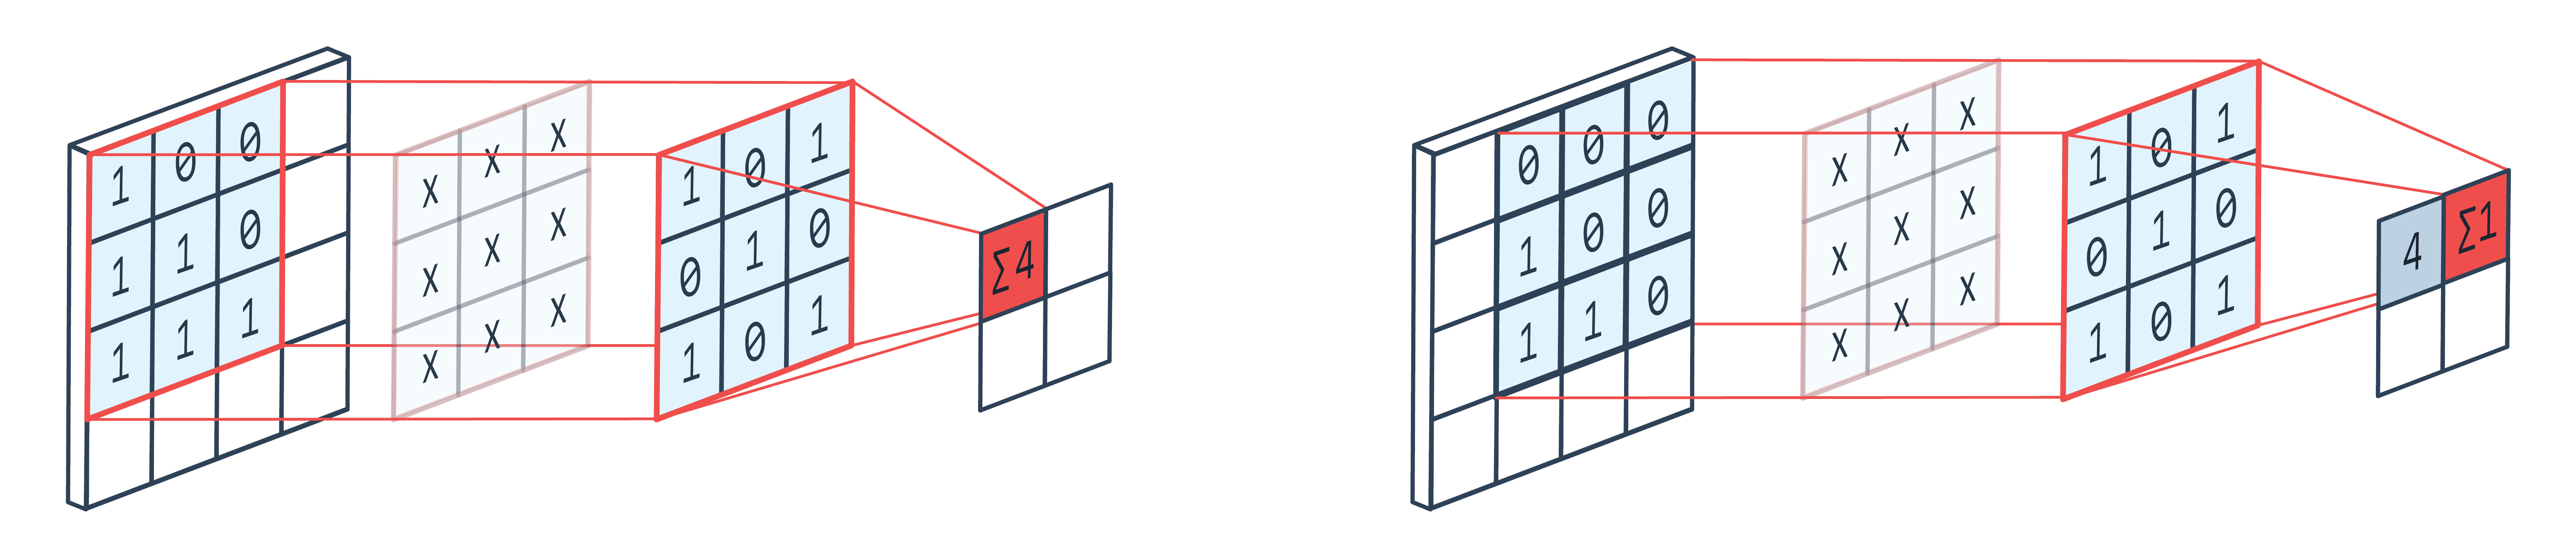
\includegraphics[height=5cm,width=15cm]{Chapitre2/img2.png}
          \caption{Structure de Couche de convolution.}
          \label{img2}
          \end{figure}
     
     % =========== Pooling Layer ===========
     \subsubsection{Pooling Layer}   
     Ou sous-échantillonnage, Il sert généralement de médiateur entre plusieurs couches de convolution. Max-pooling et Average-pooling sont les stratégies de mise en commun les plus fréquemment utilisées dans les CNN. La mise en commun apporte de nombreux avantages aux CNN. En particulier, la mise en commun vise à empêcher le surajustement en concentrant les données locales avec une fenêtre de mise en commun réduisant ainsi la dimensionnalité des données. La réduction de la dimensionnalité des données permet également de réduire les calculs.
     \begin{figure}[H]
          \centering
          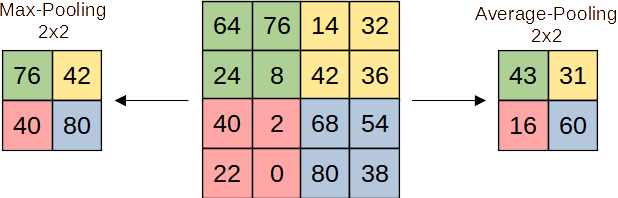
\includegraphics[height=5cm,width=15cm]{Chapitre2/img3.png}
          \caption{Max-pooling et Average-pooling.}
          \label{img3}
          \end{figure}
     
     % =========== Fully Connected Layer ===========
     \subsubsection{Fully Connected Layer (FC)}   
     Cette couche prend la sortie de convolution/polling, l'aplatit et prédit la meilleure étiquette pour décrire l'image. Comme dans un réseau neuronal à anticipation normal, les entrées de la couche entièrement connectée sont multipliées par les poids et additionnées. Ensuite, une fonction d'activation est utilisée pour produire la sortie comme Softmax qui est largement utilisée dans les problèmes de classification.
     \begin{figure}[H]
          \centering
          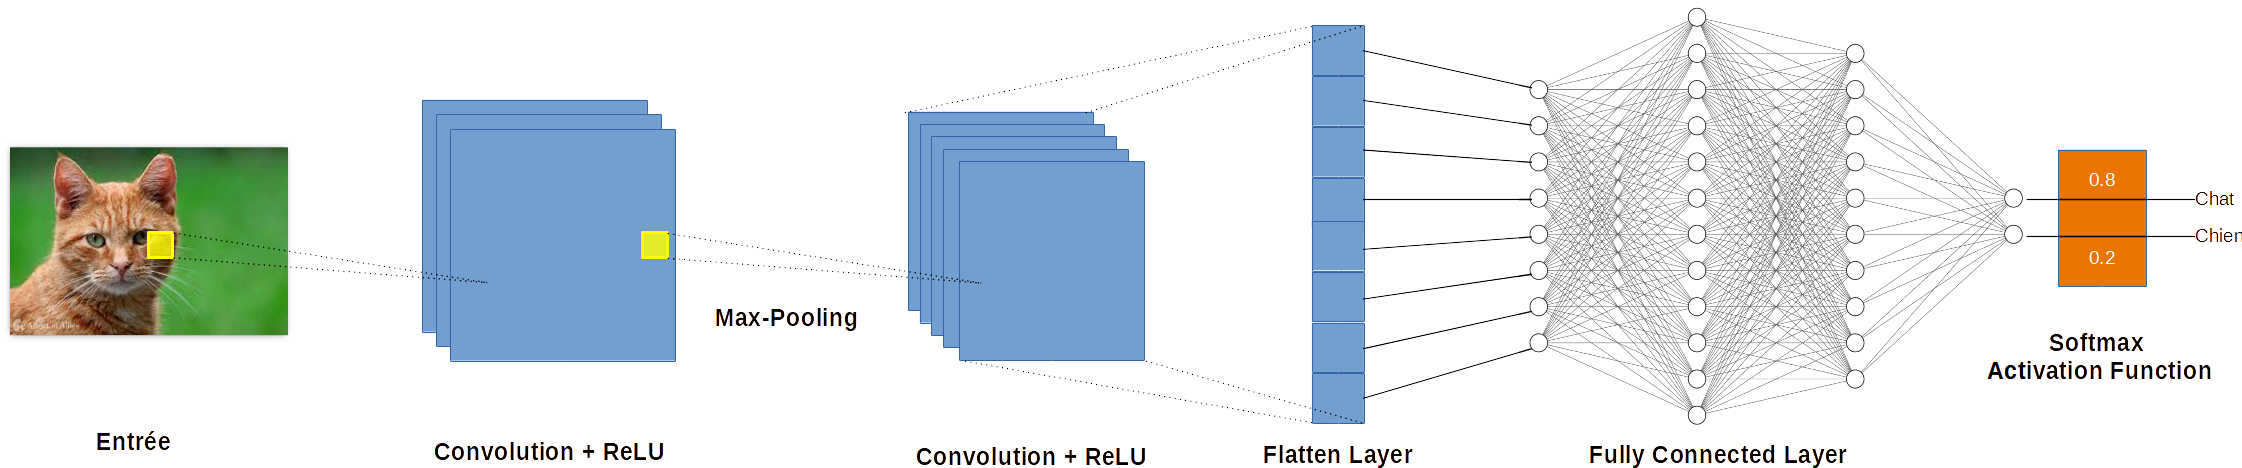
\includegraphics[height=4cm,width=18cm]{Chapitre2/img4.png}
          \caption{Exemple de structure de réseaux de neurones convolutionnels.}
          \label{img4}
          \end{figure}

% =========== Transfer Learning ===========
     \subsection{L'apprentissage par transfert} 
     L'apprentissage par transfert se produit lorsque des modèles existants sont réutilisés pour résoudre un nouveau défi ou problème. L'apprentissage par transfert n'est pas un type distinct d'algorithme d'apprentissage automatique, mais plutôt une technique ou une méthode utilisée lors de la formation de modèles. Les connaissances acquises lors des formations précédentes sont recyclées pour aider à effectuer une nouvelle tâche. La nouvelle tâche sera liée d'une certaine manière à la tâche précédemment formée.

     Le processus prend des parties pertinentes d'un modèle existant et les applique pour résoudre un problème nouveau mais similaire. Un élément clé de l'apprentissage par transfert est la généralisation. Cela signifie que seules les connaissances pouvant être utilisées par un autre modèle dans différents scénarios ou conditions sont transférées. Au lieu que les modèles soient liés de manière rigide à un ensemble de données de formation, les modèles utilisés dans l'apprentissage par transfert seront plus généralisés. Les modèles développés de cette manière peuvent être utilisés dans des conditions changeantes et avec différents ensembles de données.
     \begin{figure}[H]
          \centering
          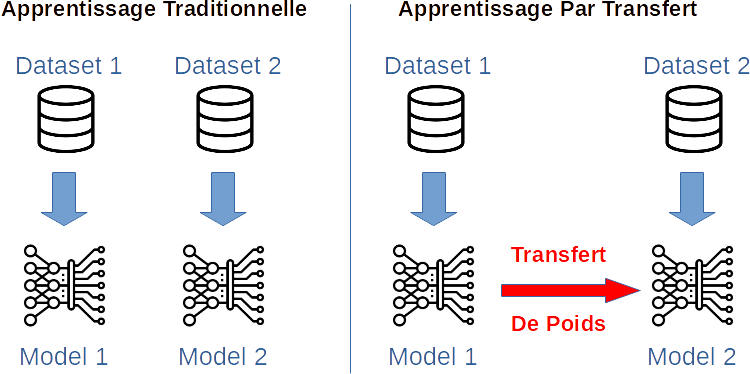
\includegraphics[height=7cm,width=13cm]{Chapitre2/img5.png}
          \caption{Différence entre l'apprentissage traditionnel et l'apprentissage par transfert.}
          \label{img5}
          \end{figure}

% =========== Backbones =========== 
     \subsection{Architectures CNN populaires} 
     Au fil des ans, de nombreuses architectures de réseaux de neurones convolutionnels ont été introduites, chacune avec sa complexité et sa profondeur uniques en termes de couches en corrélation avec les performances de l'architecture. Les plus notables sont :
     
          % =========== AlexNet =========== 
          \subsubsection{AlexNet} \cite{alexnet_paper}
          Alex Krizhevsky en collaboration avec Ilya Sutskever et Geoffrey Hinton. en 2012, a développé un réseau de neurones convolutifs composé de 8 couches, dont 5 sont convolutives et 3 sont entièrement connectées. Le réseau s'appelle AlexNet. il a amélioré LeNet-5 en ajoutant plus de couches et en contenant environ 60 millions de paramètres. Les unités linéaires rectifiées (ReLU) sont utilisées pour la première fois comme activations dans AlexNet au lieu des activations sigmoïdes et tanh pour ajouter de la non-linéarité.
          \begin{figure}[H]
               \centering
               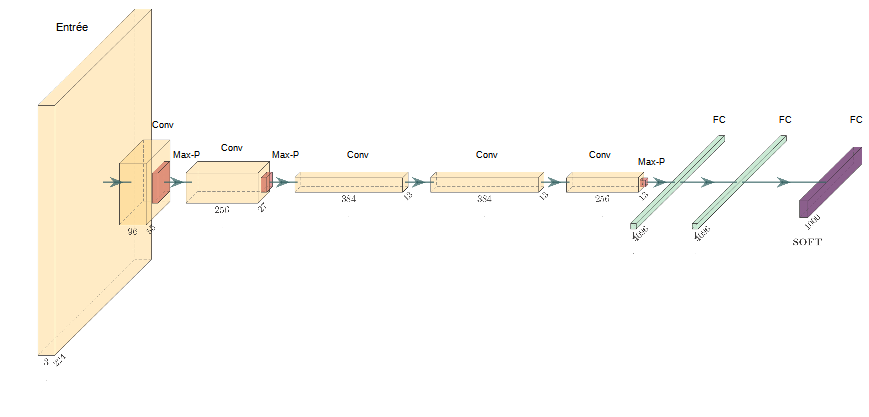
\includegraphics[height=9cm,width=15cm]{Chapitre2/img6.png}
               \caption{Architecture de AlexNet.}
               \label{img6}
               \end{figure}

          % =========== VGG-16 ===========
          \subsubsection{VGG-16} \cite{vgg_paper}
          est l'une des architectures les plus utilisées dans la détection d'objets et a 	réalisé des performances intéressantes, elle est sortie en 2014, composée de 13 couches convolutives et 3 entièrement connectées avec activation ReLU. VGG-16 fournit plus de couches par rapport à AlexNet et utilise des filtres plus petits de 2x2 et 3x3. Il comprend 138 millions de paramètres.
          \begin{figure}[H]
               \centering
               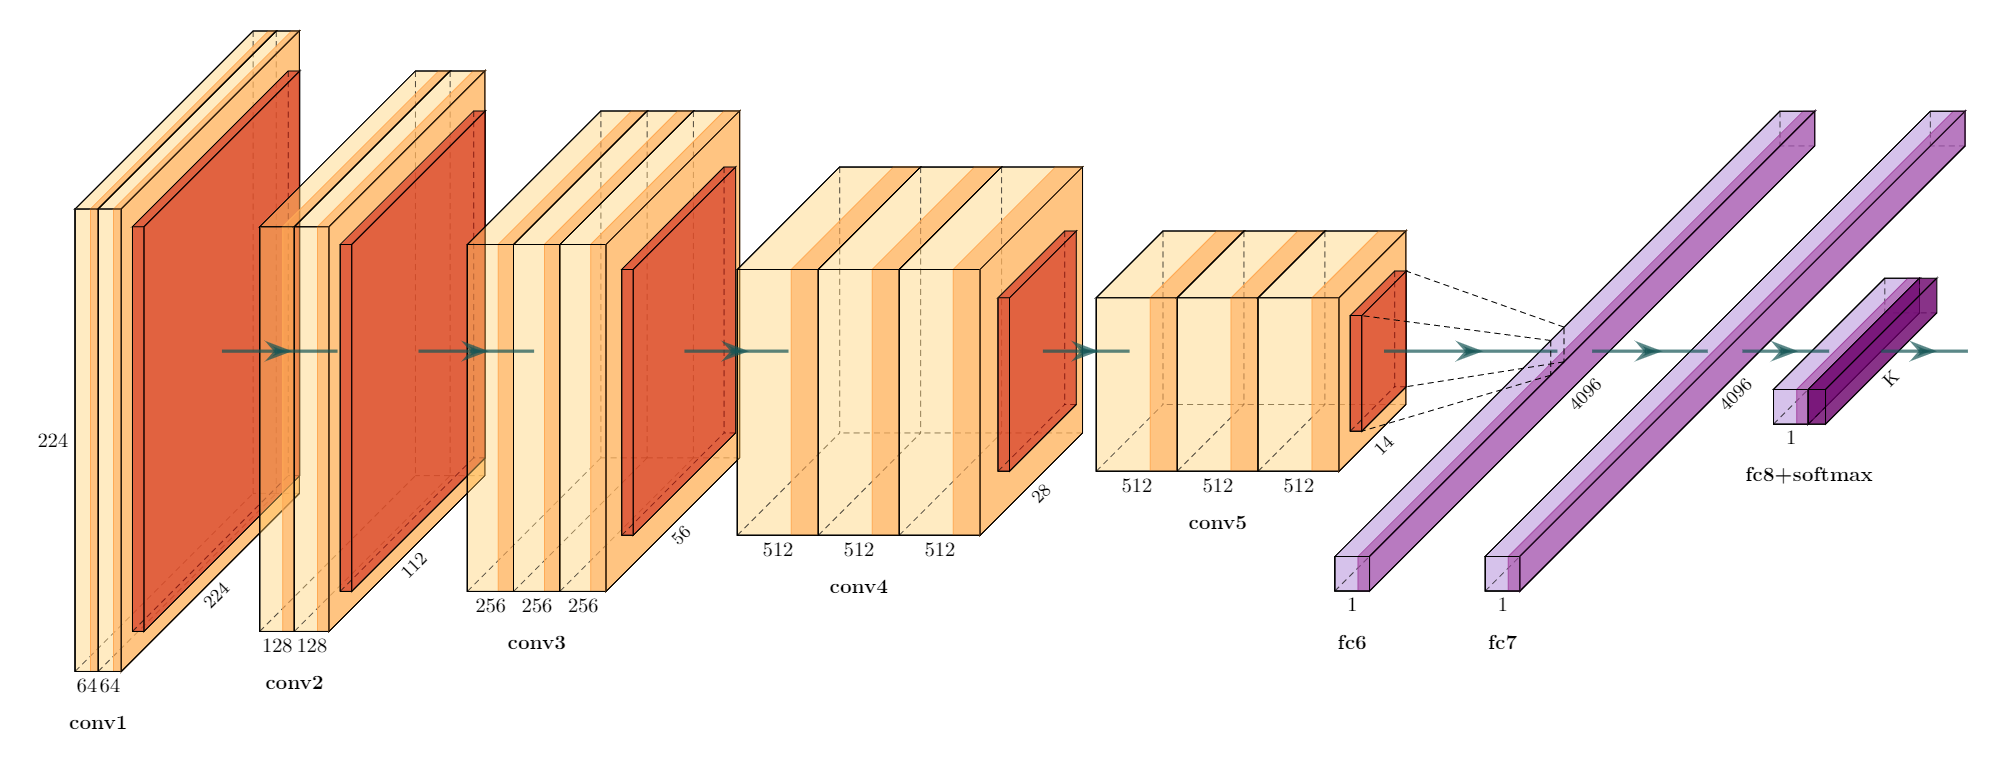
\includegraphics[height=9cm,width=15cm]{Chapitre2/img7.png}
               \caption{Architecture de VGG-16.}
               \label{img7}
               \end{figure}

          % =========== ResNet ===========
          \subsubsection{ResNet} \cite{resnet_paper}
          Les réseaux de neurones convolutifs sont devenus de plus en plus profonds avec l'ajout de couches, mais une fois la précision saturée, elle chute rapidement, ce phénomène appelé dégradation. Pour résoudre ce problème, He et al. en 2015 ont développé des ResNets basés sur les résidus. Les résidus sont essentiellement des connexions de raccourci, une pile de couches définies de telle sorte que la sortie d'une couche est prise et ajoutée à une autre couche plus profonde dans le réseau. Étant donné que le module d'apprentissage résiduel résout le problème de la dégradation de la formation, la profondeur du réseau est augmenté et les performances sont continuellement améliorées.

          Il existe de nombreuses variantes de ResNets, par exemple, ResNet-50 qui est composé de 26 millions de paramètres, ResNet-101 avec 44 millions de paramètres et ResNet-152 qui est plus profond avec 152 couches, les deux sont largement utilisés dans la détection d'objets.
          \begin{figure}[H]
               \centering
               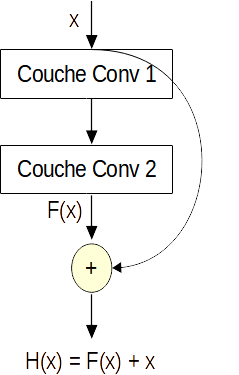
\includegraphics[height=8cm,width=5cm]{Chapitre2/img8.png}
               \caption{Structure d'un bloc résiduel.}
               \label{img8}
               \end{figure}
          
          % =========== GoogLeNet ===========
          \subsubsection{GoogLeNet} \cite{googlenet_paper}
          Aussi appelé Inception V1, GoogLeNet est un petit réseau développé par Szegedy et al. en 2014. Leur méthode est différente de celle de VGGNet et AlexNet. Ils ont proposé une nouvelle notion connue sous le nom Inception Block, où elle intègre des transformations convolutives à plusieurs échelles. Inception Block comprend des filtres de différentes tailles 1x1, 3x3 et 5x5. Il utilise une convolution 1x1 au milieu du réseau pour réduire la dimensionnalité et ils ont choisi d'utiliser Max-Pooling au lieu de couches entièrement connectées. Le réseau est composé de 22 couches avec 5 millions de paramètres. GoogLeNet est principalement utilisé dans le modèle de détection d'objets YOLO.
          \begin{figure}[H]
               \centering
               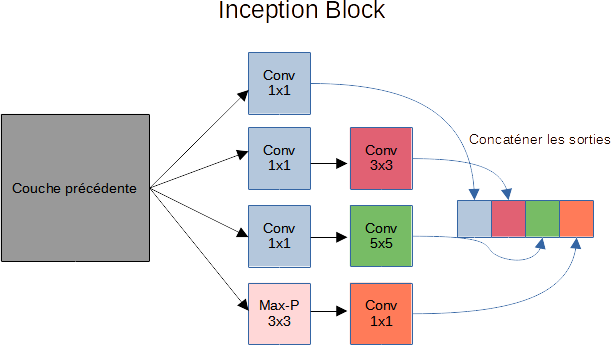
\includegraphics[height=8cm,width=12cm]{Chapitre2/img9.png}
               \caption{Structure de Inception Block.}
               \label{img9}
               \end{figure}

           % =========== Darknet-53 ===========
           \subsubsection{Darknet-53} \cite{yolov3_paper}
           Il a été introduit en 2018 par Joseph Redmon Ali Farhadi, il sert d'architecture de YOLOv3. c'était une amélioration de son prédécesseur Darknet-19 qui était l'architecture de YOLOv2. il se compose de 53 couches convolutionnelles qui servent de base au réseau de détection d'objets ou à un extracteur de caractéristiques. inclure l'utilisation de connexions résiduelles. Après chaque couche convolutive, un groupe résiduel a différents blocs résiduels tels que 1x, 2x, 4x et 8x. Pour sous-échantillonner la dimension spatiale des cartes d'entités, une convolution striée avec une foulée de 2 est utilisée avant chaque groupe résiduel. Cela a permis d'éviter la perte de fonctionnalités de bas niveau et d'encoder des informations de position utiles pour la détection d'objets.
           \begin{figure}[H]
                \centering
                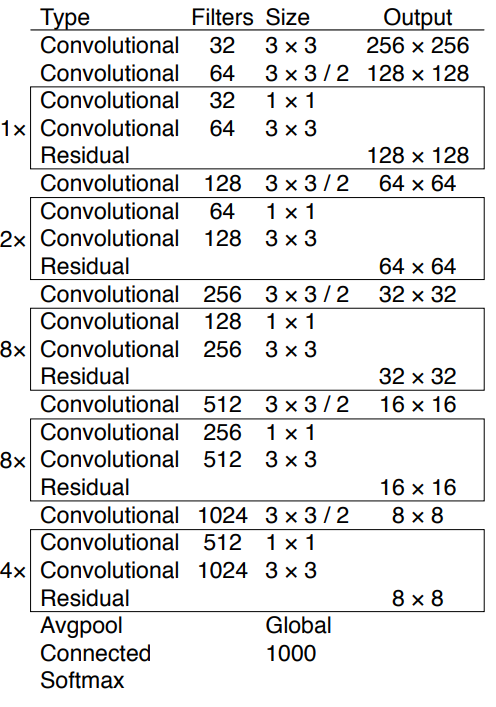
\includegraphics[height=8cm,width=7cm]{Chapitre2/img10.png}
                \caption{Architecture de Darknet-53.}
                \label{img10}
                \end{figure}



% =========== Loss Functions ===========
\section{Fonction de perte pour la détection d'objet}
En Apprentissage profond, la fonction de perte est aussi appelée fonction de coût. L'objectif principal de la fonction de perte est de mesurer l'écart entre la valeur prédite du réseau et la valeur réelle de l'échantillon. Plus la valeur de la fonction de perte est petite, meilleur est l'apprentissage du modèle de réseau, ce qui prouve la convergence et la robustesse du modèle de réseau. La détection d'objet est divisée en classification d'objet et localisation d'objet. Par conséquent, la fonction de perte inclut la perte de classification et la perte de localisation. La perte de classification appartient à la classification et la perte de localisation appartient à la régression de la boîte englobante.

     % =========== Classification Loss ===========
     \subsection{Perte de Classification}
          % =========== Hing Loss ===========
          \subsubsection{Hinge loss}
          est une fonction proxy de la fonction de perte $0-1$. Il peut être utilisé comme perte pour le problème de marge maximale dans l'apprentissage automatique ou l'apprentissage en profondeur, et peut être étendu à la perte SVM multi-classes. Plus la valeur après sommation est petite, plus le score de la classe d'erreur sera.
          \begin{center} $L(y)=\sum_{j \neq i}max(0,y_j-y_i+1)$ \end{center}

          Où $y_j$ est le score des autres classes et $y_i$ le score réel declasse.	

          % =========== Cross entropy loss ===========
          \subsubsection{Cross entropy loss}
          est également appelée perte de log, qui est utilisée dans le classificateur softmax. La fonction de softmax est de convertir la caractéristique dimensionnelle $(k+1)\times1$ en distribution de probabilité dimensionnelle $(k+1)\times1$. La valeur d'indice de la probabilité maximale est l'étiquette de catégorie de l'échantillon prédit. Par conséquent, selon les caractéristiques de la fonction softmax.
          \begin{center} $L(p,u)=-\sum_{i=0}^{k}u_i log p_i$ \end{center}
          où $p=(p_0,..., p_k)$ est la distribution de probabilité de $K+1$ catégories calculées par le softmax, et u est la véritable étiquette de catégorie. La structure de la fonction montre que la perte d'entropie croisée est la distance entre la valeur prédite et la valeur réelle cible. La structure de la fonction a une optimisation convexe, qui a une bonne convergence lors de la descente du gradient. Il est plus adapté à la classification multi-catégories qu'à Hing loss.

     % =========== Localisation Loss ===========
     \subsection{Perte de Localistaion}
          % =========== Squared Loss ===========
          \subsubsection{Squared Loss}
          est l'une des fonctions de perte de base de la régression de la boîte englobante, également connue sous le nom de perte $L_2$. Il représente la somme des carrés des différences entre la valeur cible et la valeur prédite.
          \begin{center} $L(y, f(x)) = (y - f(x))^2$ \end{center}

          % =========== RSS ===========
          \subsubsection{Residual Sum of Squares (RSS)}
          également connue sous le nom de somme des carrés des résidus (SSR) ou somme des carrés de l'estimation des erreurs (SSE), est la somme des carrés des résidus (écarts prédits par rapport aux valeurs empiriques réelles des données). Il s'agit d'une mesure de l'écart entre les données et un modèle d'estimation, tel qu'une régression linéaire.
          \begin{center} $L(Y, F(X)) = \sum_{i=1}^{n}(y_i - f(x_i))^2$ \end{center}

          % =========== MSE ===========
          \subsubsection{Mean Squared Error (MSE)}
          mesure la quantité d'erreur dans les modèles statistiques. Il évalue la différence quadratique moyenne entre les valeurs observées et prédites. Lorsqu'un modèle n'a pas d'erreur, le MSE est égal à zéro. À mesure que l'erreur du modèle augmente, sa valeur augmente. L'erreur quadratique moyenne est également appelée écart quadratique moyen (MSD).
          \begin{center} $L(Y, F(X)) = \frac{1}{n}\sum_{i=1}^{n}(y_i - f(x_i))^2$ \end{center}

          % =========== Absolute loss ===========
          \subsubsection{Absolute loss}
          est la fonction de perte pour la régression de la boîte englobante, également appelée $L_1$. La différence entre la perte $L_1$ et la perte $L_2$ est que $L_1$ représente la somme des valeurs absolues de la différence entre la valeur cible et la valeur prédite.
          \begin{center} $L(y, f(x))=|y-f(x)|$ \end{center}

          % =========== SAD ===========
          \subsubsection{Sum of Absolute Differences (SAD)}
          S'il y a n échantillons avec $L_1$, la fonction de perte prend la forme suivante
          \begin{center} $L(Y, f(X))=\sum_{i=1}^{n}|y_i-f(x_i)|$ \end{center}

          % =========== MAE ===========
          \subsubsection{Mean Absolute Error (MAE)}
          La valeur moyenne de SAD est généralement utilisée comme perte de régression, appelée erreur absolue moyenne (MAE)
          \begin{center} $L(Y, f(X))=\frac{1}{n}\sum_{i=1}^{n}|y_i-f(x_i)|$ \end{center}

          La perte $L_1$ et la perte $L_2$ ont leurs propres avantages et inconvénients lorsqu'elles sont utilisées pour la régression de la boîte englobante.
          La perte $L_1$ est plus robuste aux valeurs aberrantes, mais elle a des points où la dérivée ne peut pas être déduite, ce qui rend la descente de gradient inefficace.
          La descente de gradient de la perte $L_2$ est plus précise et simple à calculer, mais plus sensible aux valeurs aberrantes.
          Par conséquent, les avantages de la perte $L_1$ et de la perte $L_2$ sont combinés dans la conception de la fonction de perte de régression de la boîte englobante.

% =========== Proposal generation ===========
\section{Génération de proposition}
     La génération de proposition joue un rôle très important dans la détection d'objet. Un générateur de proposition génère un ensemble de rectangles englobants, qui sont potentiellement des objets. Ces propositions sont ensuite utilisées pour le raffinement de la classification et de la localisation. 
     
     Notamment, les détecteurs à un étage et les détecteurs à deux étages génèrent des propositions, la principale différence est que les détecteurs à deux étages génèrent un ensemble clairsemé de propositions avec uniquement des informations de premier plan ou d'arrière-plan, tandis que les détecteurs à un étage considèrent chaque région de l'image comme un potentiel. proposition, et estime en conséquence la classe et les coordonnées de la boîte englobante des objets potentiels à chaque emplacement.
     
     % =========== Traditional computer vision methods ===========
     \subsection{Méthodes traditionnelles de vision par ordinateur}
     Ces méthodes génèrent des propositions en images en utilisant les méthodes de vision par ordinateur basées sur des indices de bas niveau, tels que les bords, coins, couleur, etc. 

     Le principal avantage de ces méthodes est qu'elles sont très simples et peuvent générer des propositions avec un rappel élevé. Cependant, ces méthodes sont principalement basées sur des repères visuels de bas niveau tels que la couleur ou les contours. Ils ne peuvent pas être optimisés conjointement avec l'ensemble du pipeline de détection. Ainsi, ils sont incapables d'exploiter la puissance des ensembles de données à grande échelle pour améliorer l'apprentissage de la représentation.

     \subsubsection{Score d'objectivité} les méthodes basées sur la prédiction d'un score d'objectivité de chaque boîte candidate mesurant la probabilité qu'elle contienne un objet.
     \subsubsection{Superpixels fusionnant} est basé sur la fusion de superpixels générés à partir des résultats de segmentation. Selective Search \cite{selctive_search_paper} était un algorithme de génération de propositions basé sur la fusion de super-pixels. Il a calculé les multiples segments hiérarchiques générés par la méthode de segmentation, qui ont été fusionnés en fonction de leurs facteurs visuels (couleur, zones, etc.), et enfin des cadres de délimitation ont été placés sur les segments fusionnés.
     \subsubsection{Segmentation des semences} commence par plusieurs régions de départ, et pour chaque départ, des segments de premier plan et d'arrière-plan sont générés. Pour éviter de créer une segmentation hiérarchique, CPMC \cite{cpmc_paper} a généré un ensemble de segments superposés initialisés avec diverses graines. Chaque segment de proposition était la solution d'un problème de segmentation binaire (avant-plan ou arrière-plan).

     % =========== Anchor-based methods ===========
     \subsection{Méthodes basées sur des ancres}
     Une grande famille de générateurs de propositions supervisés est celle des méthodes basées sur des ancres. Ils génèrent des propositions basées sur des hors pré-définis. Ren et al. propose un réseau de proposition de région (RPN) \cite{rcnn_paper} pour générer des propositions de manière supervisée sur la base de cartes de caractéristiques convolutives profondes. Le réseau a glissé sur toute la carte des caractéristiques à l'aide de filtres de convolution 3 × 3. Pour chaque position, k ancres (ou estimations initiales des boîtes englobantes) de tailles et de rapports d'aspect variables ont été prises en compte. Ces tailles et ratios permettaient de faire correspondre des objets à différentes échelles dans l'ensemble de l'image. Sur la base des boîtes de liaison de vérité au sol, les emplacements des objets ont été mis en correspondance avec les ancres les plus appropriées pour obtenir le signal de supervision pour l'estimation de l'ancre. Un vecteur de caractéristiques à 256 dimensions a été extrait de chaque ancre et a été introduit dans deux branches sœurs : la couche de classification et la couche de régression. La branche de classification était responsable de la modélisation du score d'objectivité tandis que la branche de régression encodait quatre valeurs réelles pour affiner l'emplacement de la boîte englobante à partir de l'estimation d'origine de l'ancre. Sur la base de la vérité terrain, chaque ancre a été prédite comme étant soit un objet, soit simplement un arrière-plan par la branche de classification.
     \begin{figure}[H]
          \centering
          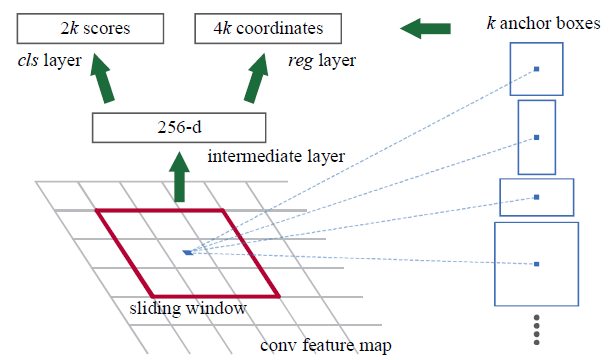
\includegraphics[height=7cm,width=14cm]{Chapitre2/img18.png}
          \caption{Réseau de proposition de région \cite{diagram_rpn_overflow}}
          \label{img18}
          \end{figure}

     % =========== Keypoints-based methods ===========
     \subsection{Méthodes basées sur les points clés}
     \subsubsection{Méthodes basées sur les coins} prédire les cadres de délimitation en fusionnant des paires de coins apprises à partir de la carte d'entités. Denet \cite{denet_paper} a reformulé le problème de détection d'objets de manière probabiliste. Pour chaque point sur la carte des caractéristiques, Denet a modélisé la distribution d'être l'un des 4 types d'objets d'angle (en haut à gauche, en haut à droite, en bas à gauche, en bas à droite) et appliqué un classificateur bayésien naïf sur chaque coin des objets pour estimer le score de confiance d'une boîte englobante. Cet algorithme basé sur les coins a éliminé la conception des ancres et est devenu une méthode plus efficace pour produire des propositions de haute qualité.
     \subsubsection{Méthodes basées sur le centre} la probabilité d'être le centre des objets est prédite sur chaque position de la carte d'entités, et la hauteur et la largeur sont directement en régression sans aucun a priori d'ancrage.

% =========== Feature representation learning ===========
\section{Apprentissage de la représentation des caractéristiques}
L'apprentissage de la représentation des caractéristiques est un élément essentiel de l'ensemble du cadre de détection. Les objets cibles se trouvent dans des environnements complexes et présentent une grande variation d'échelle et de rapports d'aspect.

     % =========== Multi-scale feature learning ===========
     \subsection{Apprentissage de fonctionnalités multi-échelles}
     Les algorithmes de détection d'objets typiques basés sur des réseaux convolutifs profonds n'utilisent qu'une carte de caractéristiques à une seule couche pour détecter les objets. Les réseaux convolutionnels profonds apprennent des caractéristiques hiérarchiques dans différentes couches qui capturent des informations à différentes échelles. Plus précisément, les caractéristiques des couches peu profondes avec des informations riches en espace ont une résolution plus élevée et des champs récepteurs plus petits et sont donc plus adaptées à la détection de petits objets, tandis que les caractéristiques riches en sémantique dans les couches profondes sont plus robustes.à l'éclairage, à la translation et ont des champs récepteurs plus grands, et sont plus adaptés à la détection de gros objets. Lors de la détection de petits objets, des représentations à haute résolution sont requises et la représentation de ces objets peut même ne pas être disponible dans les caractéristiques de la couche profonde, ce qui rend difficile la détection de petits objets. Ainsi, la gestion des problèmes d'échelle des caractéristiques est devenue un problème de recherche fondamental dans la détection d'objets.
     \subsubsection{Pyramide d'images} Une idée intuitive consiste à redimensionner les images d'entrée dans un certain nombre d'échelles différentes (pyramide d'images) et à entraîner plusieurs détecteurs, chacun étant responsable d'une certaine gamme d'échelles. Pendant les tests, les images sont redimensionnées à différentes échelles suivies par plusieurs détecteurs et les résultats de détection sont fusionnés.
     \subsubsection{Fonctionnalités intégrées} Une autre approche consiste à construire une seule carte d'entités en combinant des entités dans plusieurs couches et en faisant des prédictions finales basées sur la nouvelle carte construite. En fusionnant des entités de couches peu profondes spatialement riches et des entités de couches profondes riches en sémantique, les nouvelles entités construites contiennent des informations riches et peuvent ainsi détecter des objets à différentes échelles. Ces combinaisons sont généralement réalisées en utilisant des connexions de saut. La normalisation des caractéristiques est requise car les normes des caractéristiques des différentes couches ont une variance élevée.
     \subsubsection{Pyramide de prédiction} Le SSD de Liu et al \cite{ssd_paper}. a combiné des caractéristiques grossières et fines de plusieurs couches ensemble. Dans SSD, les prédictions étaient faites à partir de plusieurs couches, chaque couche étant responsable d'une certaine échelle d'objets. Plus tard, de nombreux efforts ont suivi ce principe pour détecter des objets multi-échelles.
     \subsubsection{Pyramide des fonctionnalités} Pour combiner l'avantage des fonctionnalités intégrées et de la pyramide de prédiction, Lin et al. proposé Feature Pyramid Network (FPN) \cite{fpn_paper} qui a intégré différentes caractéristiques d'échelle avec des connexions latérales de manière descendante pour construire un ensemble de cartes de caractéristiques invariantes à l'échelle, et plusieurs classificateurs dépendants de l'échelle ont été appris sur ces pyramides de caractéristiques. Plus précisément, les caractéristiques profondes riches en sémantique ont été utilisées pour renforcer les caractéristiques peu profondes riches en espace. Ces caractéristiques descendantes et latérales ont été combinées par sommation ou concaténation élément par élément, avec de petites convolutions réduisant les dimensions. FPN a montré une amélioration significative de la détection d'objets, ainsi que d'autres applications, et a obtenu des résultats de pointe dans l'apprentissage de fonctionnalités multi-échelles.

     % =========== Region feature encoding ===========
     \subsection{Codage des caractéristiques régionales}
     Pour les détecteurs à deux étages, le codage des caractéristiques de région est une étape critique pour extraire les caractéristiques des propositions dans des vecteurs de caractéristiques de longueur fixe. Dans R-CNN, Girshick et al. \cite{rcnn_paper} propositions de régions recadrées à partir de l'image entière et redimensionnement des régions recadrées en patchs de taille fixe (224 × 224) via une interpolation bilinéaire, suivie d'un extracteur de caractéristiques de convolution profonde. Leur méthode encodait des caractéristiques de région à haute résolution, mais le calcul était coûteux. La couche ROI Pooling a été proposée pour coder les caractéristiques de la région. Le ROI Pooling a divisé chaque région en nxn cellules (par exemple 7x7 par défaut) et seul le neurone avec le signal maximum passerait à l'étape d'anticipation. Ceci est similaire à la mise en commun maximale, mais dans des régions de tailles (potentiellement) différentes. ROI Pooling a extrait les fonctionnalités de la carte de fonctionnalités sous-échantillonnée et, par conséquent, a eu du mal à gérer les petits objets.

     % =========== Contextual reasoning ===========
     \subsection{Raisonnement contextuel}
     Les informations textuelles jouent un rôle important dans la détection d'objets. Les objets ont souvent tendance à apparaître dans des environnements spécifiques et coexistent parfois aussi avec d'autres objets. Pour chaque exemple, les oiseaux volent couramment dans le ciel. L'utilisation efficace des informations contextuelles peut aider à améliorer les performances de détection, en particulier pour détecter des objets avec des repères insuffisants (petit objet, occlusion, etc.). Apprendre la relation entre les objets avec leur contexte environnant peut améliorer la capacité du détecteur à comprendre le scénario. 
     \subsubsection{Raisonnement contextuel global} fait référence à l'apprentissage du contexte dans l'ensemble de l'image. Contrairement aux détecteurs traditionnels qui tentent de classer des régions spécifiques de l'image en tant qu'objets, l'idée ici est d'utiliser les informations contextuelles (c'est-à-dire les informations du reste de l'image) pour classer une région d'intérêt particulière. Par exemple, détecter une balle de baseball à partir d'une image peut être difficile pour un détecteur traditionnel (car il peut être confondu avec des balles d'autres sports); mais si les informations contextuelles du reste de l'image sont utilisées (par exemple, terrain de baseball, joueurs, batte), il devient plus facile d'identifier l'objet balle de baseball.
     \subsubsection{Raisonnement du contexte de la région} encode les informations contextuelles entourant les régions et apprend les interactions entre les objets avec leur environnement. Modéliser directement les relations entre différents emplacements et catégories d'objets avec le contexte est très difficile. Chen et al. ont proposé Spatial Memory Network (SMN) \cite{smn_paper} qui a introduit un module basé sur la mémoire spatiale. Le module de mémoire spatiale a capturé des contextes au niveau de l'instance en assemblant des instances d'objet dans des représentations pseudo « image » qui ont ensuite été utilisées pour le raisonnement des relations d'objet.

     % =========== Deformable feature learning ===========
     \subsection{Apprentissage des caractéristiques déformables}
     Un bon détecteur doit être robuste à la déformation non rigide des objets. Avant l'ère de l'apprentissage en profondeur, les modèles basés sur des pièces déformables (DPM) \cite{dpm_paper} avaient été utilisés avec succès pour la détection d'objets. Les DPM représentaient des objets par plusieurs composants à l'aide d'une méthode de codage déformable, rendant le détecteur robuste à la transformation d'objets non rigides. Afin de permettre aux détecteurs basés sur l'apprentissage en profondeur de modéliser les déformations des parties d'objets, de nombreux chercheurs ont développé des cadres de détection pour modéliser explicitement les parties d'objets.


\section{Les méthodes de détections d'objets basées sur l'apprentissage profond} 
Les méthodes actuelles de détection d'objets sont divisées en 2 catégories :
% =========== Two-Stage ===========
     \subsection{Détecteurs à Deux-étapes}
     Ce type de détecteurs sépare la tâche de localisation d'objets de la tâche de classification d'objets. Il génère d'abord la proposition de région, puis classe la région. Le principal avantage est la haute précision de détection et le principal inconvénient est la lenteur vitesse de détection.
     
     % =========== RCNN ===========
     \subsubsection{RCNN} \cite{rcnn_paper}
     Il a été introduit par Ross Girshick et al en 2004. Il extrait d'abord 2000 régions de l'image et on les appelle des propositions de région en utilisant un algorithme de recherche sélective. Ces 2000 propositions de régions candidates sont déformées en un carré et introduites dans un réseau neuronal convolutionnel qui produit un vecteur de caractéristiques de 4096 dimensions en sortie. Le CNN agit comme un extracteur de caractéristiques et la couche dense de sortie se compose des caractéristiques extraites de l'image et les caractéristiques extraites sont introduites dans un SVM pour classer la présence de l'objet dans cette proposition de région candidate. La régression de la boîte englobante et la suppression non maximale (NMS) seront effectuées pour effectuer un réglage fin de la boîte englobante.
     \begin{figure}[H]
          \centering
          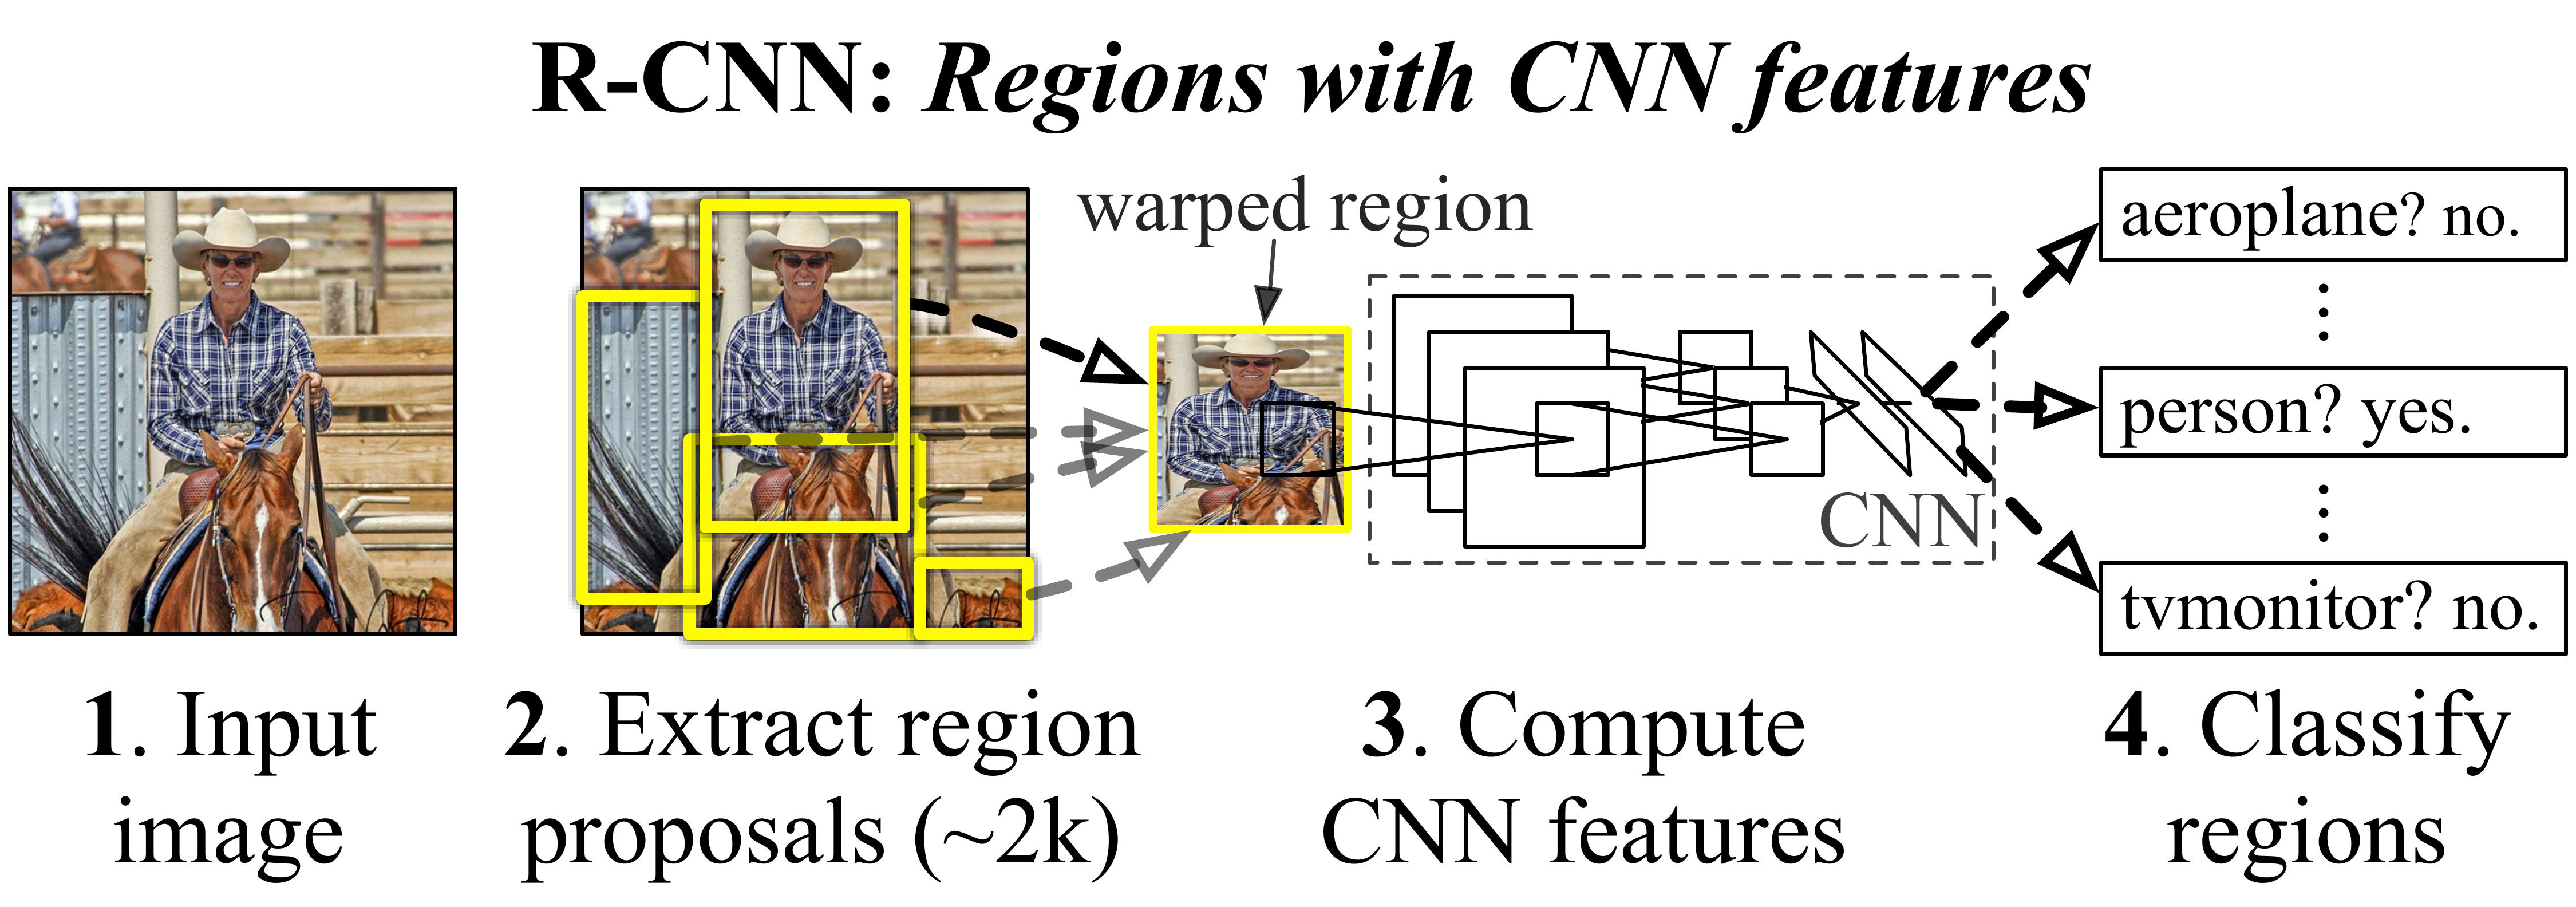
\includegraphics[height=5cm,width=15cm]{Chapitre2/img11.jpg}
          \caption{Architecture de RCNN}
          \label{img11}
          \end{figure}
     \begin{figure}[H]
          \centering
          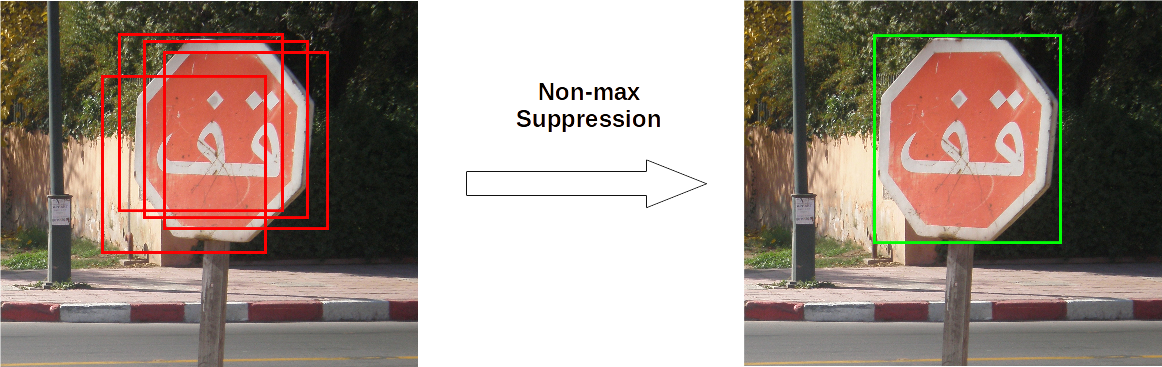
\includegraphics[height=5cm,width=15cm]{Chapitre2/img12.png}
          \caption{Suppression non maximale (NMS).}
          \label{img12}
          \end{figure}

     % =========== Fast-RCNN ===========
     \subsubsection{Fast-RCNN} \cite{fast_rcnn_paper}
     R.Girshick et al. a proposé couche de pooling de région d'intérêt (Region of Interst, ROI),il mappe différentes régions de caractéristiques sur des vecteurs de caractéristiques de taille fixe et les envoie à la couche entièrement connectée (FC). puis le softmax prédit les catégories d'objets et la régression de la boîte englobante localise avec précision l'emplacement de l'objet. Un autre changement est qu'il utilise la perte multi-tâches conjointement pour former la classification et la régression de la boîte englobante, ce qui augmente considérablement la vitesse.
     \begin{figure}[H]
          \centering
          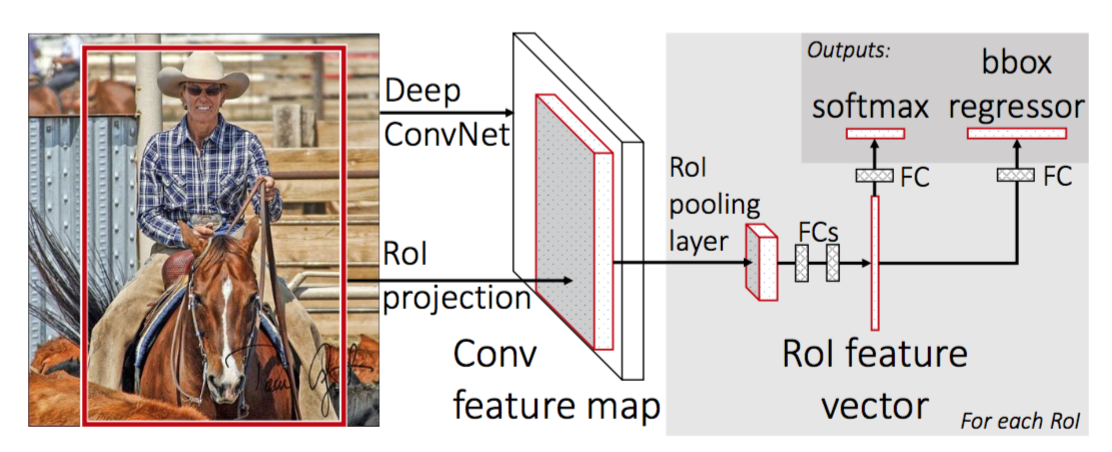
\includegraphics[height=5cm,width=15cm]{Chapitre2/img13.png}
          \caption{Architecture de Fast-RCNN}
          \label{img13}
          \end{figure}

     % =========== Faster-RCNN ===========
     \subsubsection{Faster-RCNN} \cite{faster_rcnn_paper}
     RCNN et Fast-RCNN avaient un goulot d'étranglement qui est l'algorithme de recherche sélective qui est utilisé dans la phase de proposition de région. il doit rechercher toutes les propositions de région dans l'image et les mapper dans les cartes d'entités, ce qui prend beaucoup de temps. Par conséquent, Shaoqing Ren et al ont proposé un réseau de proposition régional (RPN), il s'est intégré dans le réseau qui partage les caractéristiques de convolution de l'image complète avec le réseau de détection qui a permis au RPN d'être implémenté dans le GPU, ce qui a donné un coût quasi nul de exécution. RPN prend en entrée la carte de caractéristiques de convolution générée par la couche dorsale et génère les ancres générées par la convolution de fenêtre coulissante appliquée sur la carte de caractéristiques d'entrée.
     \begin{figure}[H]
          \centering
          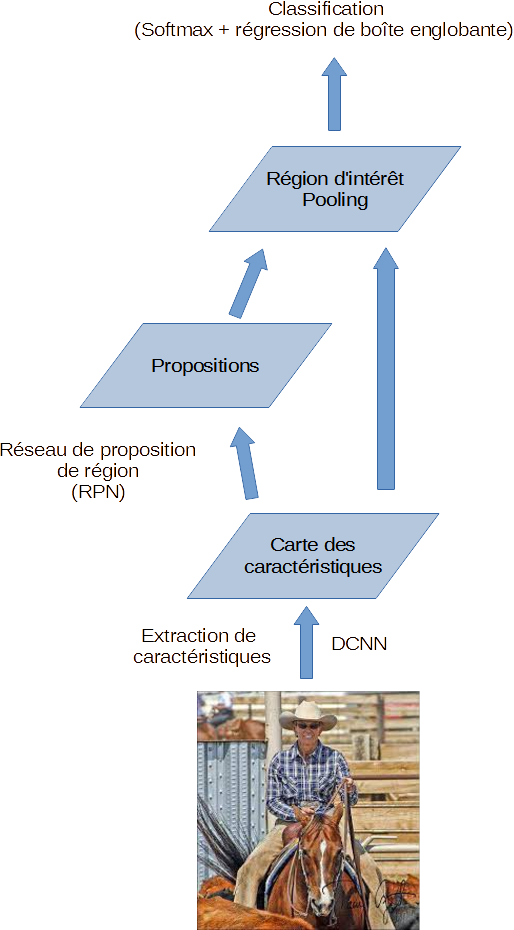
\includegraphics[height=14cm,width=7cm]{Chapitre2/img14.png}
          \caption{Architecture de Faster-RCNN}
          \label{img14}
          \end{figure}

% =========== One-Stage ===========
     \subsection{Détecteurs à Un-étapes}
     Contrairement aux détecteurs à deux étapes, ces modèles ignorent l'étape de proposition de région des modèles à deux étages et exécutent la détection directement sur un échantillonnage dense d'emplacements. Ils considèrent généralement toutes les positions sur l'image comme des objets potentiels et essaient de classer chaque région d'intérêt comme arrière-plan ou comme objet cible.

     % =========== YOLO ===========
     \subsubsection{YOLO (You Only Look Once)} \cite{yolo_paper}
     a été publié pour la première fois par Joseph Redmon et al. en 2015, le réseau utilisé utilise un GoogLeNet modifié comme réseau backbone. il se compose de 24 couches convolutionnelles et de 2 couches entièrement connectées avec une entrée réseau de 448 × 448 images. Il divise l'image complète en grilles S×S. Chaque cellule de grille est responsable de la détection du centre de l'objet tombant dans la cellule de grille. Chaque cellule de la grille prédit les probabilités de classe C, les boîtes englobantes B et les scores de confiance, et l'image complète est codée pour produire le tenseur SxSx(5B+C).
     \begin{figure}[H]
          \centering
          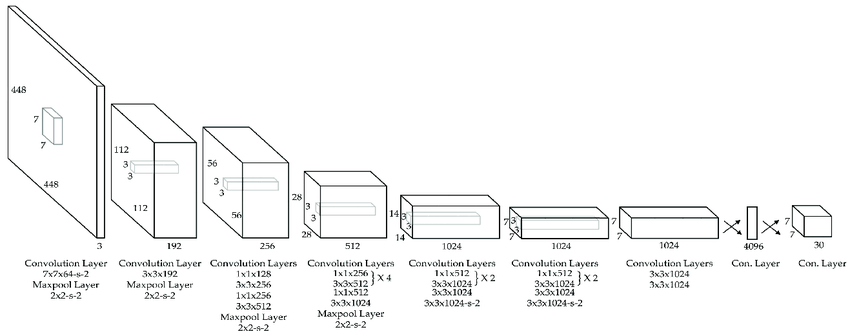
\includegraphics[height=7cm,width=14cm]{Chapitre2/img15.png}
          \caption{Architecture de YOLO (You Only Look Once)}
          \label{img15}
          \end{figure}

     % =========== YOLOv3 ===========
     \subsubsection{YOLOv3} \cite{yolov3_paper}
     été introduit par Redmon J et Farhadi A 2018, il est basé sur l'architecture Darknet-53 qui combine des blocs résiduels et FPN (Feature Pyramid Network) est un extracteur de caractéristiques qui prend une image à échelle unique d'une taille arbitraire en entrée et des sorties proportionnellement dimensionnées cartes de fonctionnalités à plusieurs niveaux, ce qui donne de bonnes performances sur une large gamme de résolutions d'entrée.
     \begin{figure}[H]
          \centering
          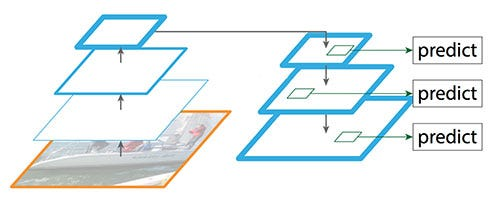
\includegraphics[height=5cm,width=9cm]{Chapitre2/img16_.jpg}
          \caption{Feature Network Pyramid (FNP)}
          \label{img16_}
          \end{figure}
     \begin{figure}[H]
          \centering
          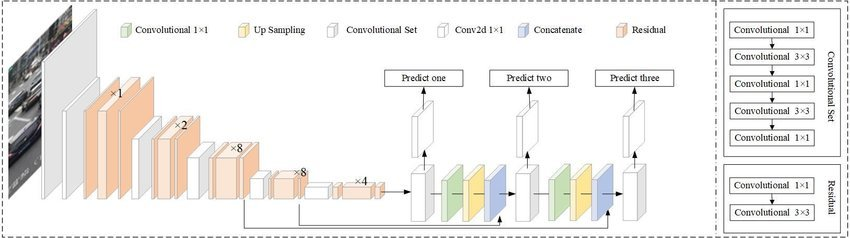
\includegraphics[height=6cm,width=14cm]{Chapitre2/img16.jpg}
          \caption{Architecture de YOLOv3}
          \label{img16}
          \end{figure}
     
          
     % =========== SSD ===========
     \subsubsection{SSD (Single Shot MultiBox Detector)} \cite{ssd_paper}
     il a été publié par C. Szegedy et al en 2016. il a utilisé VEGG16 comme réseau principal pour l'extraction de caractéristiques tout en remplaçant les couches entièrement connectées par des couches convolutives et en ajoutant 4 autres couches convolutives. Le réseau est divisé en 6 étapes. Chaque étape extrait des cartes de caractéristiques de différents niveaux sémantiques et effectue une classification d'objets et une régression par boîte englobante.
     \begin{figure}[H]
          \centering
          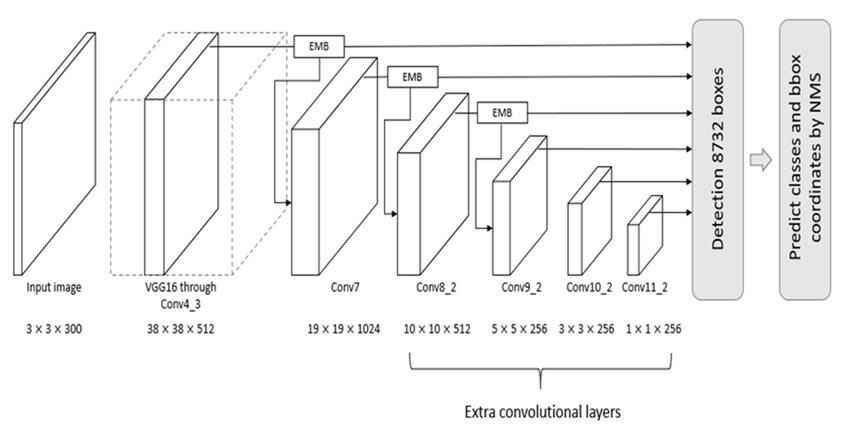
\includegraphics[height=7cm,width=14cm]{Chapitre2/img17.png}
          \caption{Architecture de SSD (Single Shot MultiBox Detector)}
          \label{img17}
          \end{figure}

% =========== Evaluation Metrics ===========
\section{Métriques pour l'évaluation des systèmes de détection d'objets} 
          % =========== IoU ===========
          \subsection{Intersection sur Union (IoU)}
          L'intersection sur l'union (IoU) est une mesure basée sur l'indice Jaccard qui évalue le chevauchement entre deux boîtes englobantes. Il nécessite une boîte englobante recherchée et une boîte englobante prédite. il peut être utilisé pour mesurer la précision de la détection d'objets.

          IoU est donnée par la zone de chevauchement entre la boîte englobante prédite et la boîte englobante recherchée terrain divisée par la zone d'union entre elles :
          \begin{figure}[H]
               \centering
               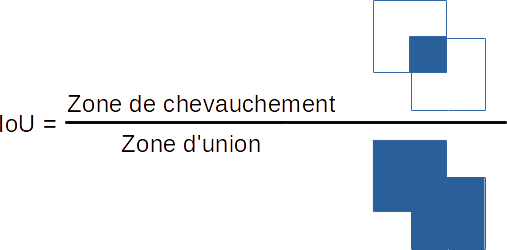
\includegraphics[height=6cm,width=14cm]{Chapitre2/img19.png}
               \caption{Intersection sur Union (IoU)}
               \label{img19}
               \end{figure}

          IoU de l'objet est plus proche de 1, la précision de détection est plus élevée.
          \begin{figure}[H]
               \centering
               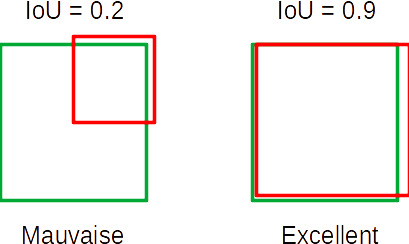
\includegraphics[height=6cm,width=10cm]{Chapitre2/img20.png}
               \caption{Exemple de Intersection sur Union (IoU)}
               \label{img20}
               \end{figure}

          % =========== Confusion Matrix ===========
          \subsection{Matrice de confusion}
          En utilisant la valeur calculée IoU avec valeur seuil prédéfinie, nous pouvons créer la matrice de confusion qui définit les performances d'un modèle en nous permettant de calculer d'autres mesures comme le rappel et la précision.
          \paragraph{Vrai positif (TP):} IoU >= seuil, une détection correcte. 
          \paragraph{Faux positif (FP):} IoU < seuil, une mauvaise détection.
          \paragraph{Faux négatif (FN):} Recherché pas trouvé.
          \paragraph{Vrai négatif (TN):} Non utilisé, il représenterait une erreur de détection corrigée. Dans la tâche de détection d'objet, il existe de nombreuses boîtes englobantes possibles qui ne doivent pas être détectées dans une image. Ainsi, TN serait toutes les boîtes englobantes possibles qui n'ont pas été correctement détectées (autant de boîtes possibles dans une image). C'est pourquoi il n'est pas utilisé par les métriques.
          
          % =========== Precision ===========
          \subsection{Précision}
          La précision est la capacité d'un modèle à identifier uniquement les objets pertinents. C'est le pourcentage de prédictions positives correctes et est donné par :
          \begin{center} $Précision = \frac{TP}{TP + FP}$ \end{center}

          % =========== Recall ===========
          \subsection{Rappel}
          Le rappel est la capacité d'un modèle à trouver tous les cas pertinents (toutes les boîtes englobantes souhaitées). C'est le pourcentage de vrais positifs détectés parmi toutes les vérités recherchées pertinentes et est donné par:
          \begin{center} $Rappel = \frac{TP}{TP + FN}$ \end{center}
          
          % =========== Precision x Recall Curve ===========
          \subsection{Précision x Rappel courbe}
          La courbe Précision x Rappel est un bon moyen d'évaluer les performances d'un détecteur d'objets car la confiance est modifiée en traçant une courbe pour chaque classe d'objets. Un détecteur d'objet d'une classe particulière est considéré comme bon si sa précision reste élevée à mesure que le rappel augmente, ce qui signifie que si vous faites varier le seuil de confiance, la précision et le rappel seront toujours élevés. Une autre façon d'identifier un bon détecteur d'objets est de rechercher un détecteur capable d'identifier uniquement les objets pertinents (0 faux positifs = haute précision), en trouvant tous les objets recherchés (0 faux négatifs = rappel élevé).
          
          Un détecteur d'objets médiocre doit augmenter le nombre d'objets détectés (augmentation des faux positifs = précision inférieure) afin de récupérer tous les objets recherchés (rappel élevé). C'est pourquoi la courbe Précision x Rappel commence généralement par des valeurs de haute précision, diminuant à mesure que le rappel augmente.
          \begin{figure}[H]
               \centering
               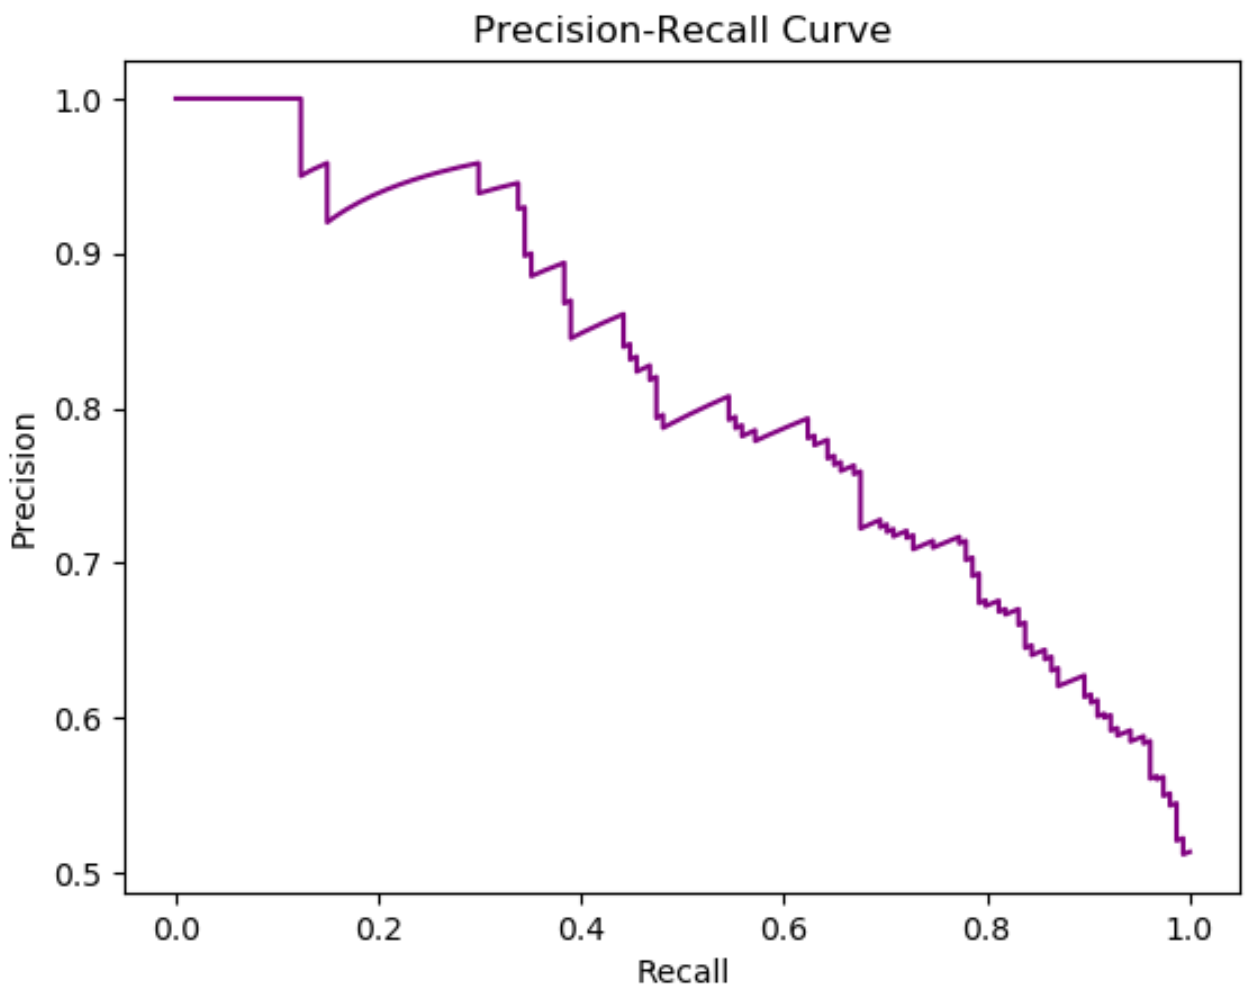
\includegraphics[height=10cm,width=12cm]{Chapitre2/img21.png}
               \caption{Exemple de Précision x Rappel courbe d'un model}
               \label{img21}
               \end{figure}
          
          % =========== AP ===========
          \subsection{Précision moyenne (AP)}
          Une autre façon de comparer les performances des détecteurs d'objets consiste à calculer l'aire sous la courbe (AUC) de la courbe Précision x Rappel. Comme les courbes AP sont souvent des courbes en zigzag qui montent et descendent, comparer différentes courbes (différents détecteurs) dans le même tracé n'est généralement pas une tâche facile car les courbes ont tendance à se croiser très fréquemment. C'est pourquoi la précision moyenne (AP), une mesure numérique, peut également nous aider à comparer différents détecteurs. En pratique, AP est la précision moyenne sur toutes les valeurs de rappel entre 0 et 1.
          
          La précision moyenne (AP) de la catégorie $C_i$ peut être calculée:
          \begin{center} $AP_{C_i} = \frac{1}{m} \sum^{m}_{j=1} P_{C_i}$ \end{center}

          % =========== mAP ===========
          \subsection{Précision moyenne moyenne  (mAP)}
          S'il existe plusieurs catégories ${C_1, C_2, ... , C_n}$ pour l'ensemble de données. Par conséquent, la précision moyenne moyenne (mAP) de l'ensemble de la catégorie peut être calculée comme suit:
          \begin{center} $mAP_{C_i} = \frac{1}{n} \sum^{n}_{j=1} P_{C_i}$ \end{center}



\section{Bases de données d'évaluation} 
Les bases de données d'évaluation jouent un rôle très crucial dans la recherche, ceux sont l'un des facteurs les plus importants pour les progrès dans le domaine, malheureusement les données sont plus difficiles et plus coûteuses à générer. Au cours de la dernière décennie, un certain nombre d'ensembles de données ont été rendus publics pour évaluer les algorithmes de détection d'objets. Ces ensembles de données sont collectés à partir de différents scénarios et peuvent donc être utilisés comme référence pour les applications. Ci-dessous, nous décrivons les ensembles de données  les plus populaires utilisés pour l'évaluation dans ce domaine:

\begin{itemize}
\item Microsoft COCO \cite{db1}
\item ImageNet \cite{db2}
\end{itemize}



\section{Conclusion} 
